\documentclass[]{article}
\usepackage[german]{babel}
\usepackage[utf8]{inputenc}
\usepackage{graphicx}
\usepackage{caption}
\usepackage{subcaption}
\usepackage{lastpage}
\usepackage{epstopdf}
\graphicspath{outdir=/u/mhemmer/Documents/Theses/BachelorArbeit/}
\usepackage{fancyhdr}
\usepackage{amsmath}
\usepackage{amsthm}
\usepackage{amsbsy}
\usepackage{amssymb}
\usepackage{hyperref}


\pagestyle{headings}
\fancyhf{}
\setcounter{section}{-1}								%Gliederungsnummerierung faengt bei 0 an.

%opening
\title{Reduzierung der systematischen Unsicherheit bei der Peakeextraktion neutraler Pionen durch Monte Carlo Template Fits}
\author{Marvin Hemmer}

\begin{document}

\maketitle
\newpage
\tableofcontents
\newpage

	\section{Einleitung}

	\section{Experimenteller Aufbau}

	\section{Analyse}
	\subsection{Daten}
	\subsubsection{Datensatz}
	\subsubsection{Trigger und Cuts}
	\subsection{Peak Extraktion mit der Standard Methode}
	Messungen mit dem EMCal liefern Ort und Energie von u.a. Photonenkandidaten. Mit diesen Informationen ist es m{\"o}glich neutrale Pionen zu rekonstruieren, da ein ${\it \pi^{0}}$ zu $\left( 98.823\pm0.034\right)\%$ in zwei Photonen zerf{\"a}llt. Der Zerfall findet statistisch Verteilt nach eine Durschnitssl{\"a}nge von ${\it c\tau} = 25.5$nm vom prim{\"a}ren Vertex statt, wobei dieser mit Hilfe der ITS bestimmt.
	Mit dem Wissen, wo sich der prim{\"a}ren Vertex befindet, sowie der Ortsaufl{\"o}sung des EMCals kann der Zerfallswinkel zwischen zwei Photonenkandidaten, welche durch das EMCal detektiert wurden, bestimmt werden.
	Die Energien der beiden Photonen $E_{\gamma1}$ und $E_{\gamma2}$, sowie der Zerfallswinkel sind f{\"u}r die Berechnung der invarianten Masse erforderlich. F{\"u}r diese gilt:
	\begin{align}
	\label{eq_invmass}
	m_{inv} &= \sqrt{2E_{\gamma1}E_{\gamma2}(1-\cos\left( \theta_{\gamma\gamma}\right) )} 
	\end{align}
	Au{\ss}erdem kann aus den vorangegangenen Daten die Aufteilung des Impulses der Photonenkandidaten bestimmt werden, welche wiederum notwendig ist, um den transversalen Impuls $p_{T}$ des $\pi^{0}$ zu Kalkulieren.
	Es gilt:
	\begin{align}
	\label{eq_pt}
	p_{T\pi^{0}} &= \sqrt{\left(p_{x1}+p_{x2}\right)^{2} +\left(p_{y1}+p_{y2}\right)^{2}} 
	\end{align}
	Die Zahlen in den Indizes beziehen sich dabei auf die Nummerierung der beiden Photonen.
	
	
	\subsubsection{Rekonstruktion}
	\begin{figure}[tbp]
		\centering
		\begin{subfigure}{.5\textwidth}
			\centering
			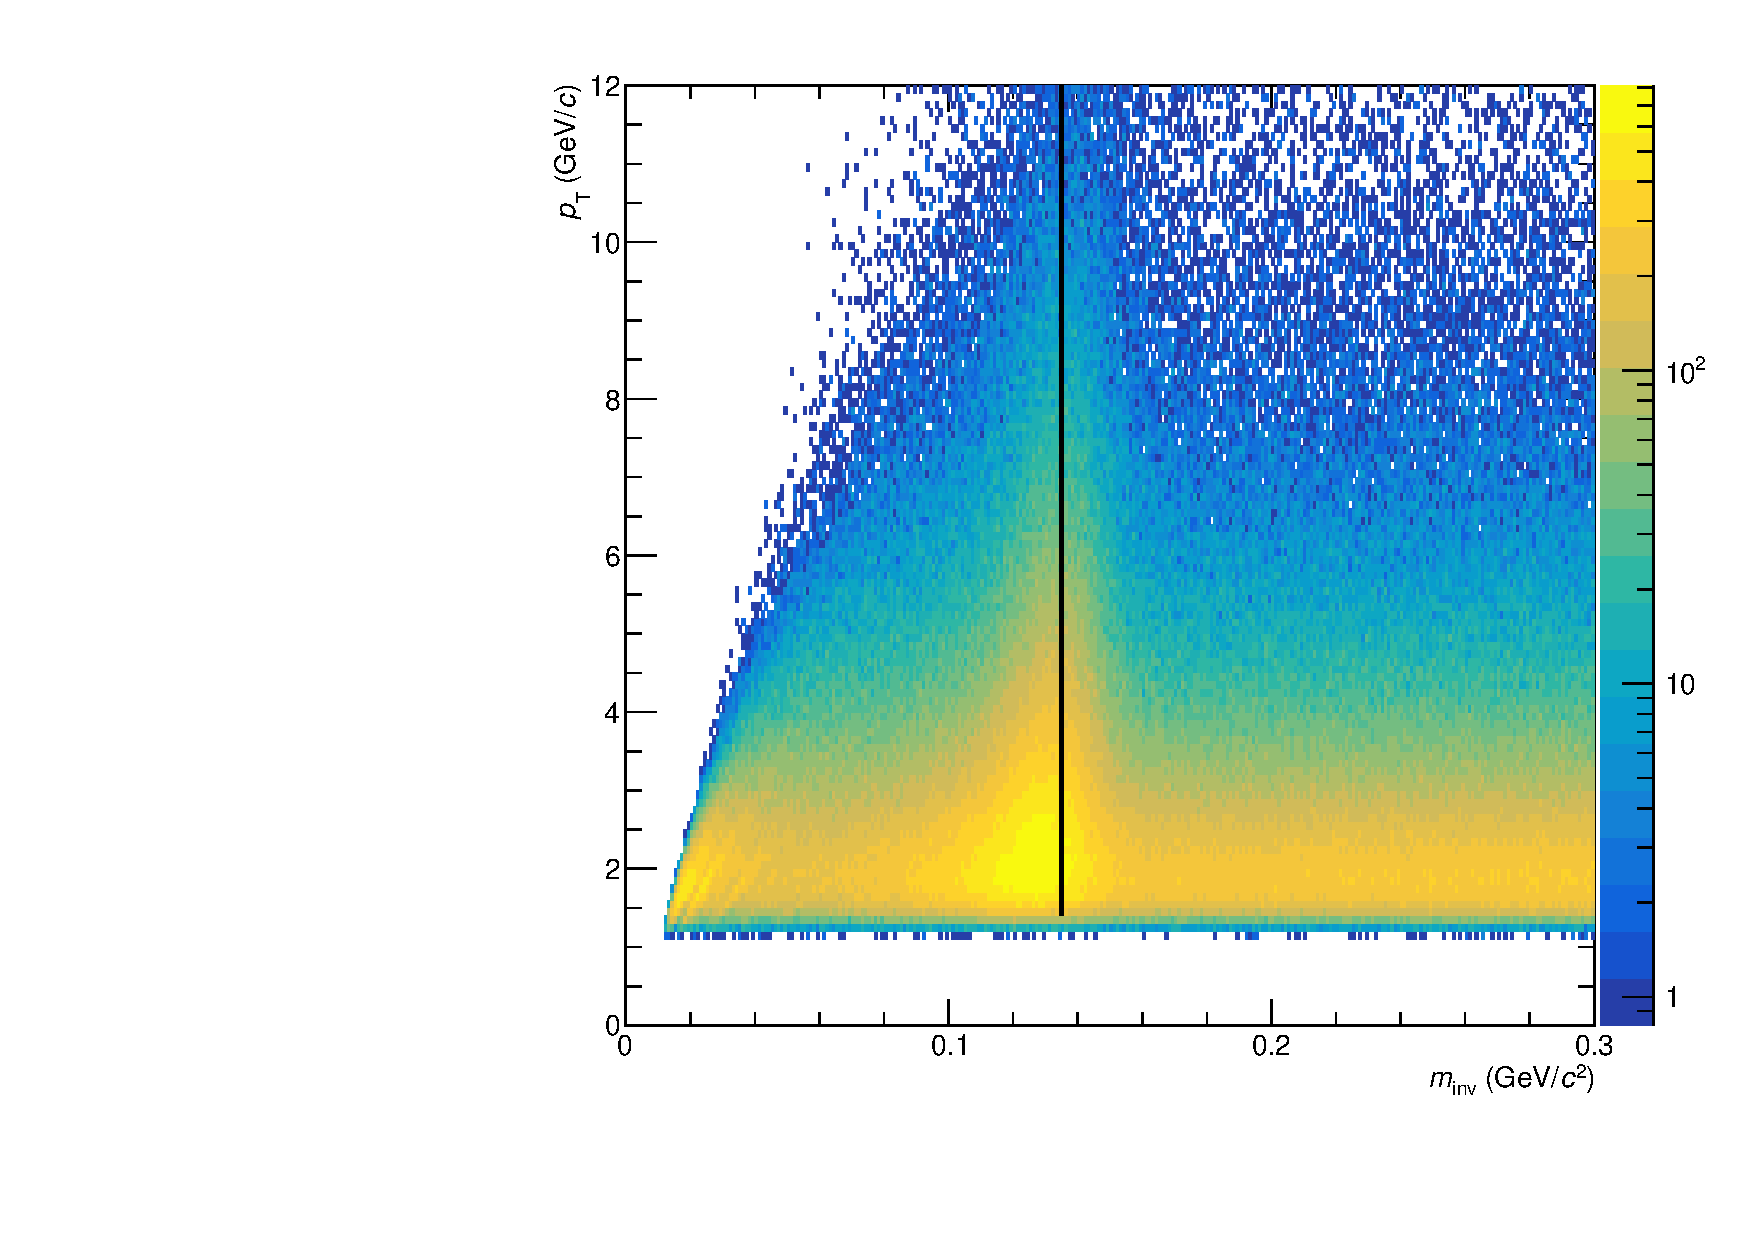
\includegraphics[width=.95\linewidth]{hInvMass_pT_Signal.pdf}
			\caption{}
			\label{figInvMassPt_a}
		\end{subfigure}%
		\begin{subfigure}{.5\textwidth}
			\centering
			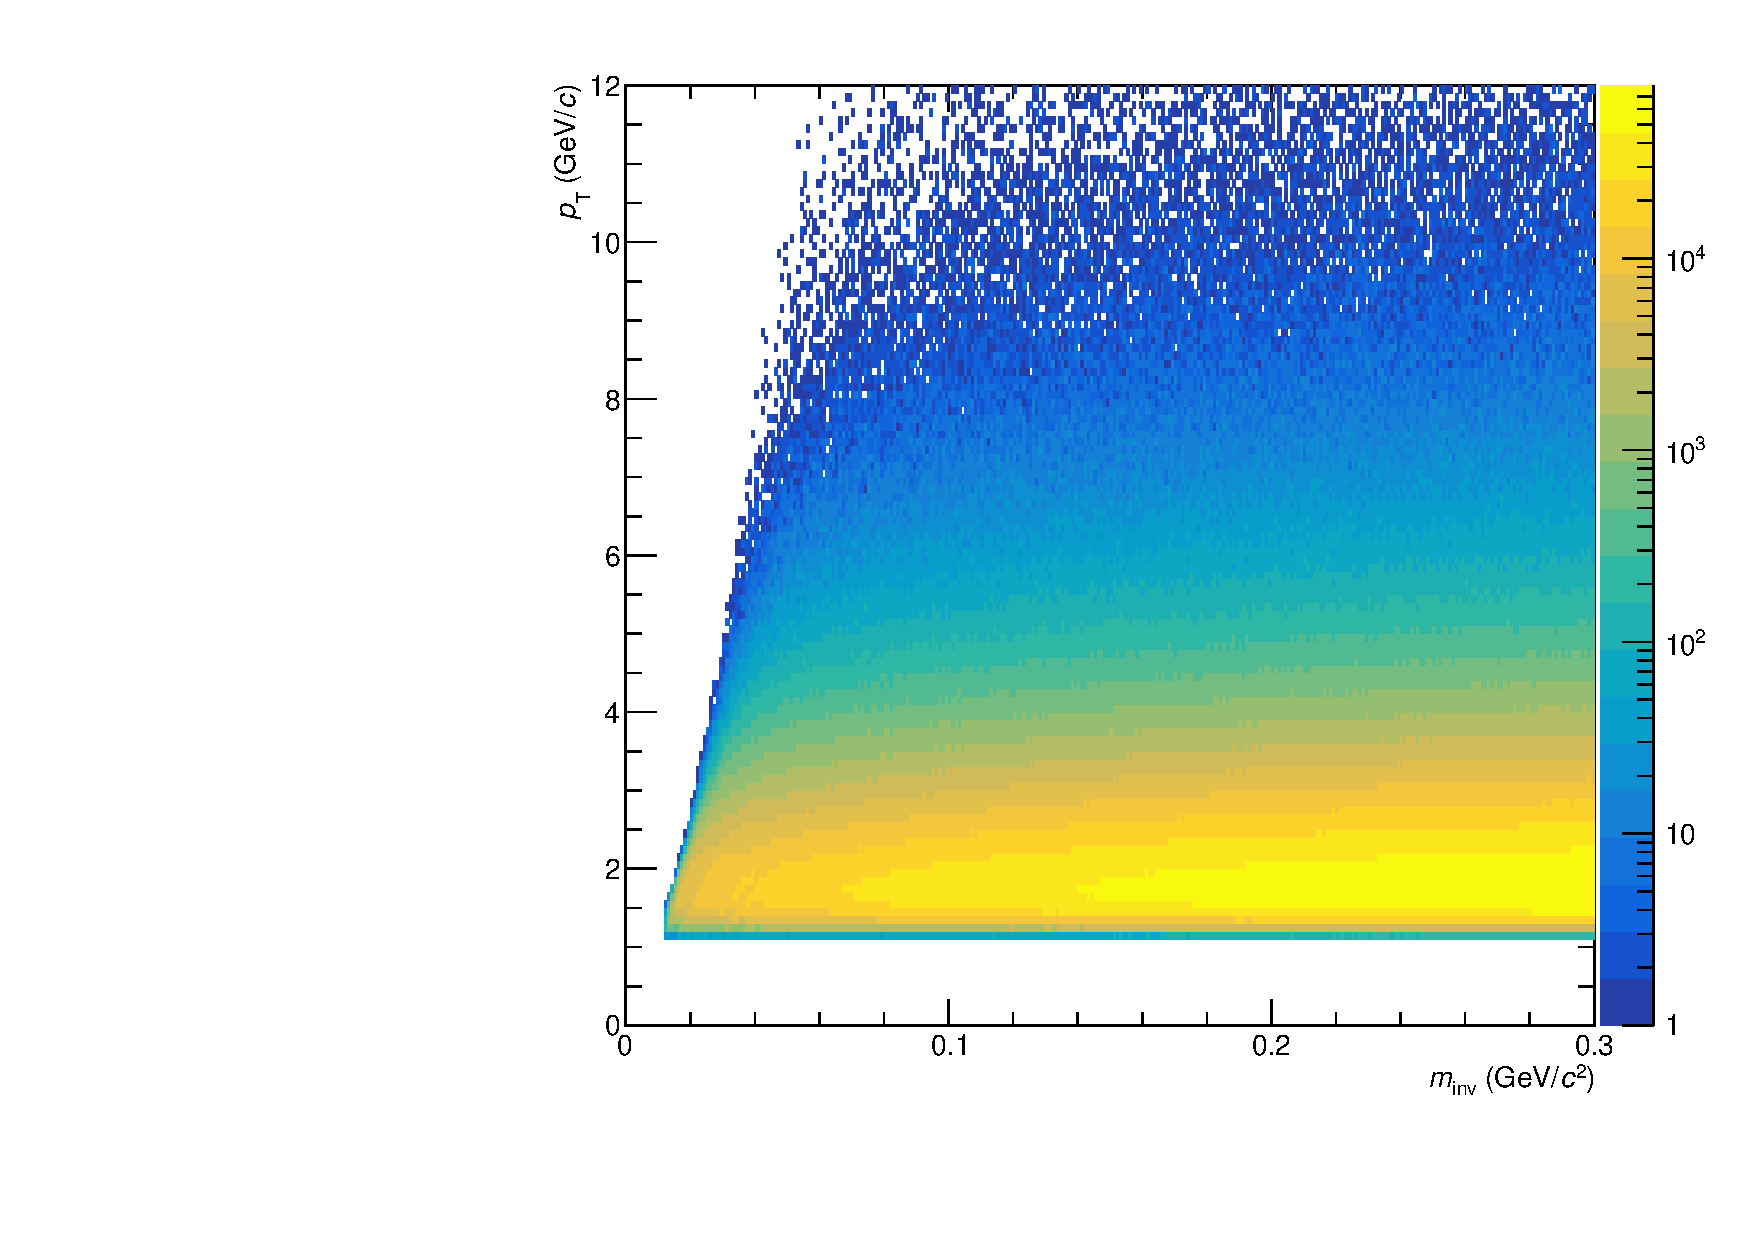
\includegraphics[width=.95\linewidth]{hInvMass_pT_Bkg.pdf}
			\caption{}
			\label{figInvMassPt_b}
		\end{subfigure}
		\caption{\newline{\bf (a)}: Rekombination von Cluster-Paaren aus jeweils der gleichen Kollision ({\it same event}). Die schwarze Linie liegt im Bereich $m_{\text{inv}}=0,135\text{ GeV/}c^{2}$, was ungef{\"a}hr der $\pi^{0}$ Masse entspricht, wo eine deutliche Peakstruktur zu Erkennen ist.\newline{\bf (b)}: Rekombination von Cluster-Paaren aus jeweils unterschiedlichen Kollision ({\it mixed event}).\newline Beides in Abh{\"a}ngigkeit der invarianten Masse, sowie des transversalen Impulses.}
		\label{figInvMassPt}
	\end{figure}

	Aus dem gew{\"a}hlten Datensatz werden alle m{\"o}glichen Kombinationen von zwei Photonenkandidaten aus der gleichen Kollision ({\it same event}) mit korrespondierendem $\theta_{\gamma\gamma}$ benutzt, um $m_{inv}$ nach \ref{eq_invmass} zu berechnen, sowie $p_{T,\pi^{0}}$ nach \ref{eq_pt} und so eine invariante Massenverteilung zu erhalten (vgl. Abbildung \ref{figInvMassPt_a}). In dieser Verteilung ist bereits eine auffallende Struktur bei $m_{inv}\approx 0.135\text{GeV/}c^{2}$ zu erkennen, welche auf richtig rekombinierte $\pi^{0}$ schlie{\ss}en l{\"a}sst. Abbildung \ref{figInvMassPt_b} zeigt eine invariante Massenverteilung bei der Photonenkandidaten aus unterschiedlichen Kollisionen ({\it mixed event}) miteinander kombiniert werden, auf welche in Kapitel \ref{sssec:num3} genauer eingegangen wird.

	\begin{figure}[tbp]
		\centering
		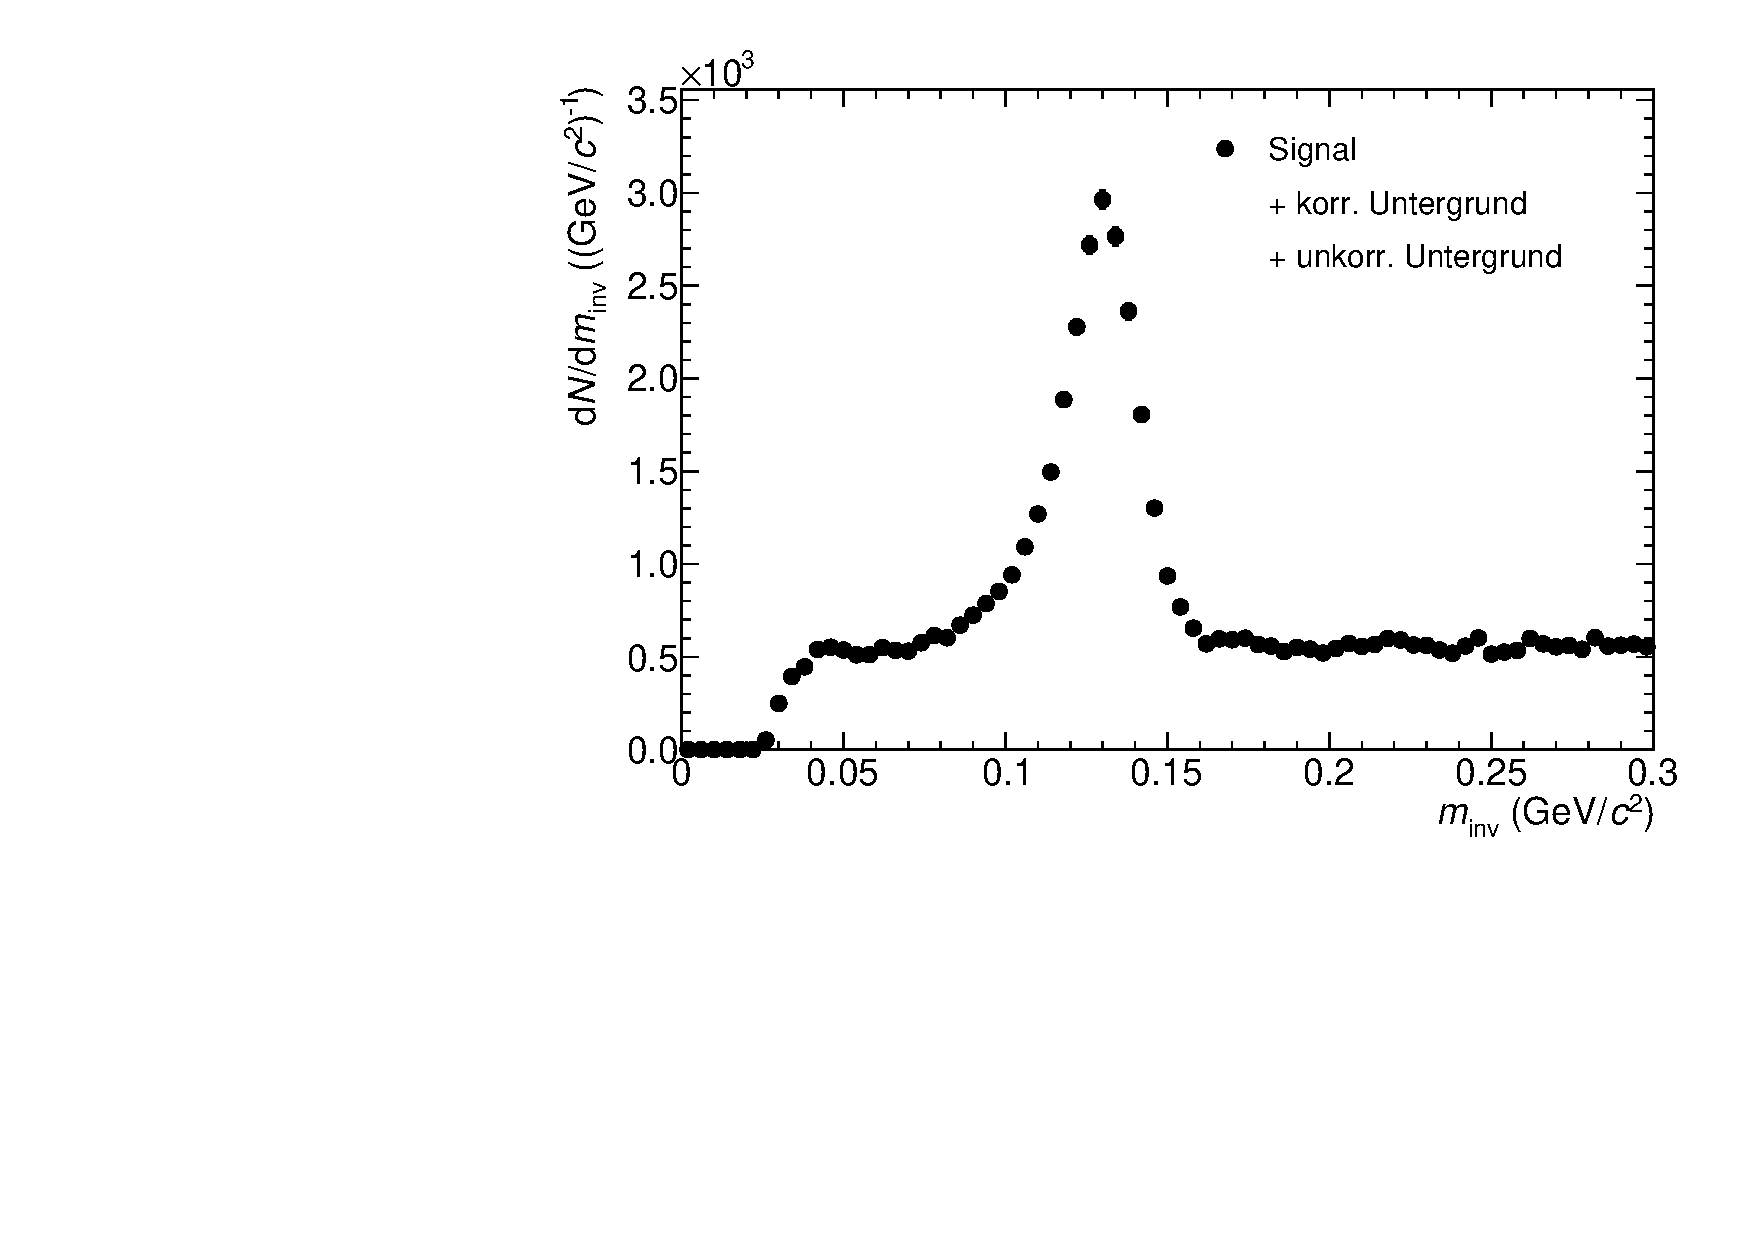
\includegraphics[width=.7\linewidth]{hSignalPlusBkg.pdf}
		\caption{Projektion von Abbildung \ref{figInvMassPt_a} im $p_{\text{T}}$-Intervall (3.2 - 3.4) $(\text{GeV/}c)$. Es ist ein deutlicher Peak um $m_{\pi^{0}} \approx 0.135\text{GeV/}c^{2}$ zu erkennen, aber auch Untergrund, da das Signal zu h{\"o}heren Massen gau{\ss}f{\"o}rmig abklingen sollte. Bei $m_{inv} < m_{\pi^{0}}$ kann Signal vorliegen, welches aus konvertierten Photonen besteht, weshalb eine Aussage {\"u}ber die Form, bzw. den Untergrund dort schwer m{\"o}glich ist.}
		\label{figSignalPlusBkg}
	\end{figure}

	Um $\pi^{0}$s in einzelnen $p_{T}$-Intervallen z{\"a}hlen zu k{\"o}nnen wird die Verteilung in entsprechende Abst{\"a}nden auf die Y-Achse projiziert. Die Intervalle werden so gew{\"a}hlt, dass sie m{\"o}glichst klein sind, w{\"a}hrend die statistischen Unsicherheiten nicht zu gro{\ss} werden. Man erh{\"a}lt Verteilungen der invarianten Masse, welche aus Signal, sowie korreliertem und unkorreliertem Untergrund bestehen (vgl. Abbildung \ref{figSignalPlusBkg}). Dennoch ist ein deutlicher Peak im Bereich der Pionenmasse von ca. 135MeV/$c^{2}$ zu erkennen. Um das Signal zu extrahieren werden im Folgende die beiden Komponenten des Untergrunds pr{\"a}sumiert.
	
	\subsubsection{Absch{\"a}tzung des unkorrelierten Untergrunds}
	\label{sssec:num3}
	
	\begin{figure}[tbp]
		\centering
		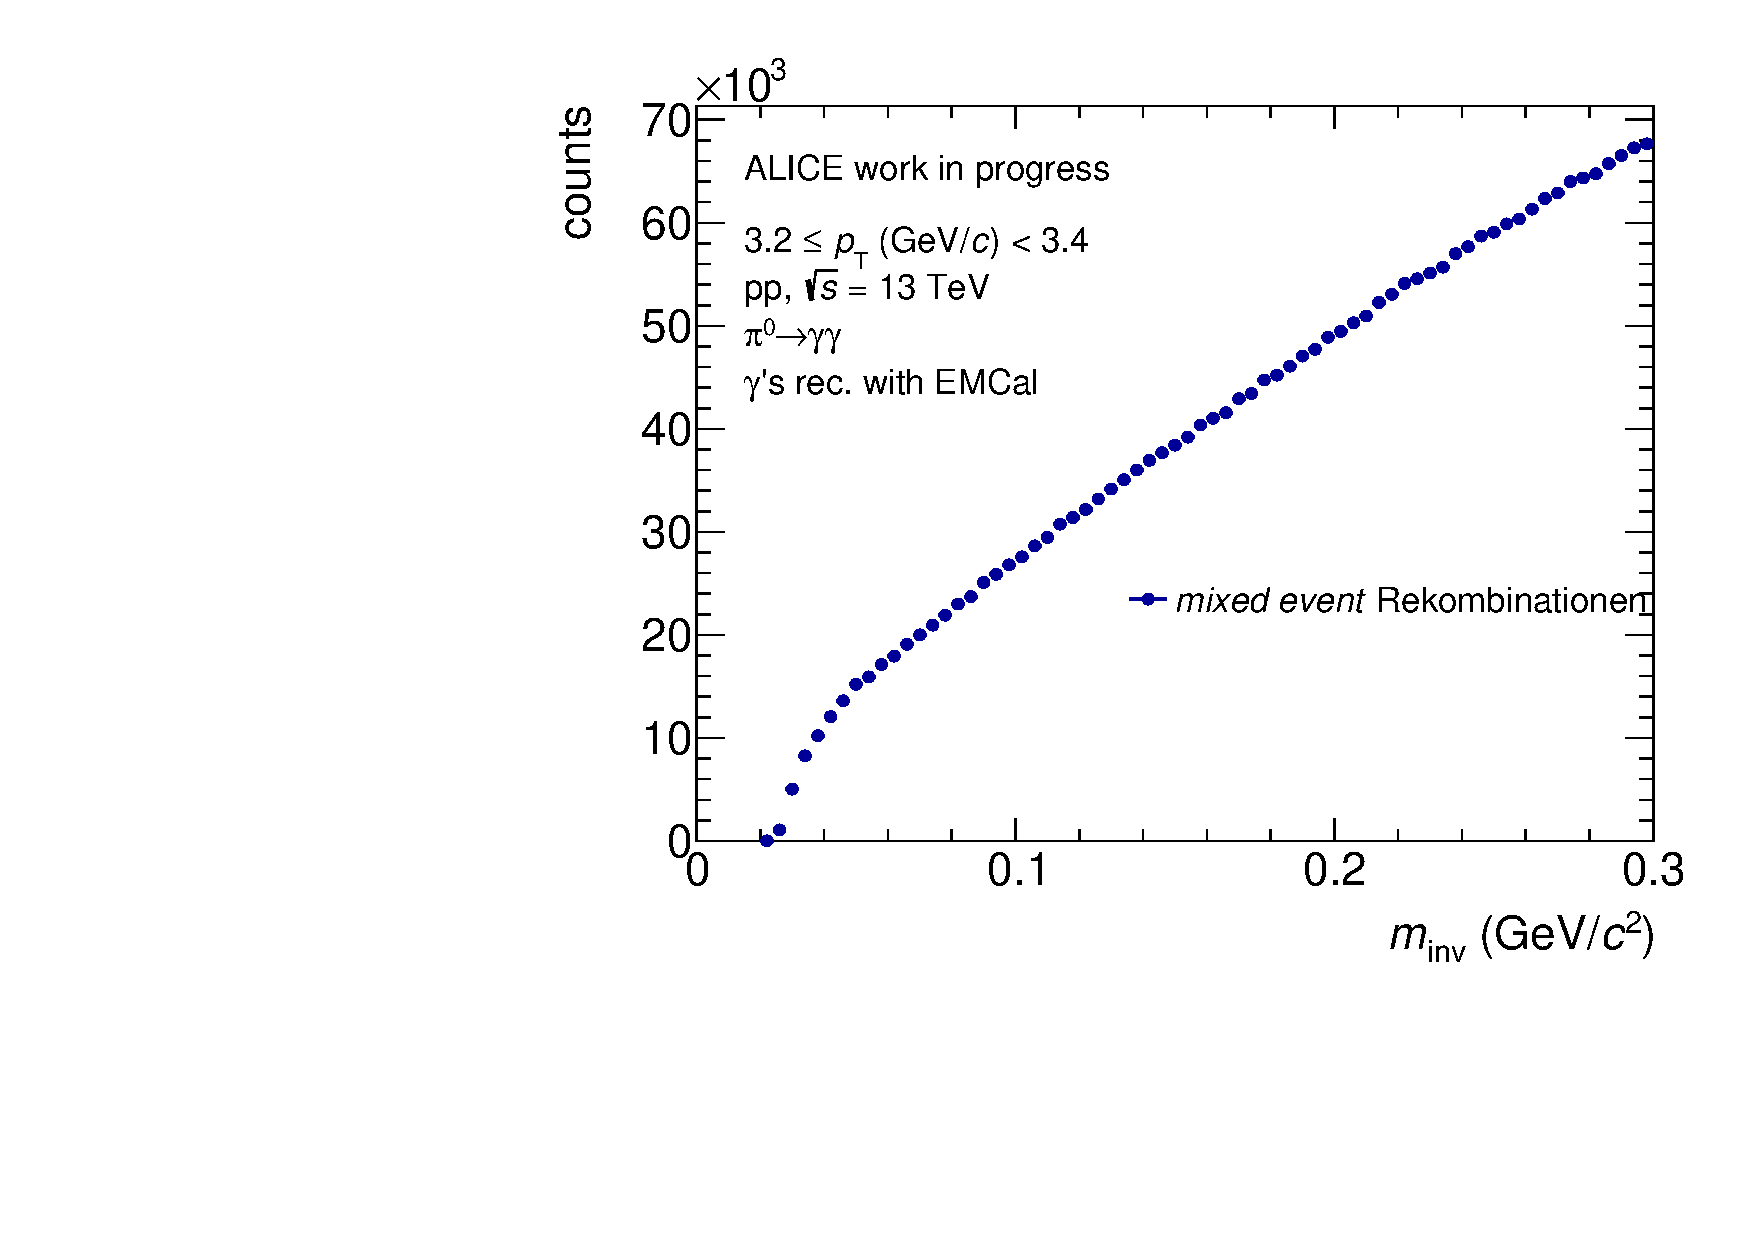
\includegraphics[width=.7\linewidth]{hUncorrBkg.pdf}
		\caption{Kombinationen von Photonenkandidaten aus unterschiedlichen Kollisionen, welche keine Korrelationen zueinander haben, weshalb auch kein Peak im Bereich der $\pi^{0}$-Masse zu sehen ist. Dies dient als Grundlage zur Bestimmung des unkorrelierten Untergrunds.}
		\label{figUncorrBkg}
	\end{figure}
	
	Durch das kombinieren aller Photonenkandidaten ist ein gro{\ss}er Anteil der rekonstruierten Massen aus nicht korreliert Paaren, da die beiden Photonenkandidaten nicht zusammenh{"a}ngen {\"u}ber beispielsweise einen Zerfall. Um diesen unkorrelierten Untergrund abzuw{\"a}gen kombiniert man im sogenannten Eventmixing Photonenkandidaten aus unterschiedlichen Events zusammen, da so sicher keine Verbindung zwischen den beiden Photonenkandidaten besteht. Abbildung \ref{figUncorrBkg} stellt das Ergebnis des Eventmixings f{\"u}r einen gew{\"a}hlten Bereich dar.
	
	Die Verteilung aus den {\it mixed events} weist keinen Peak auf und hat eine gr{\"o}{\ss}ere Anzahl Eintr{\"a}ge, als die Verteilung aus dem selben Events (vgl. Abbildung \ref{figSignalPlusBkg} und \ref{figUncorrBkg}), weshalb die mixed Event Verteilung an die der same Events skaliert werden muss. Die Skalierung erfolgt im rechten Bereich au{\ss}erhalb des $\pi^{0}$-Peaks und es ergibt sich f{\"u}r den Skalierungsfaktor:
	\begin{align}
	\label{eqBackSkalierung}
	\alpha &= \frac{\sum_{i \neq j}\sum_{n}m_{inv}\left( \gamma^{(n)}_{i},\gamma^{(n)}_{j}\right) }{\sum_{i,j}\sum_{n \neq m}m_{inv}\left( \gamma^{(n)}_{i},\gamma^{(m)}_{j}\right) }
	\end{align}
	Die oberen Indizes stehen hierbei f{\"u}r das Event, aus welchem ein Photon kommt.\newline
	
	\begin{figure}[tbp]
		\centering
		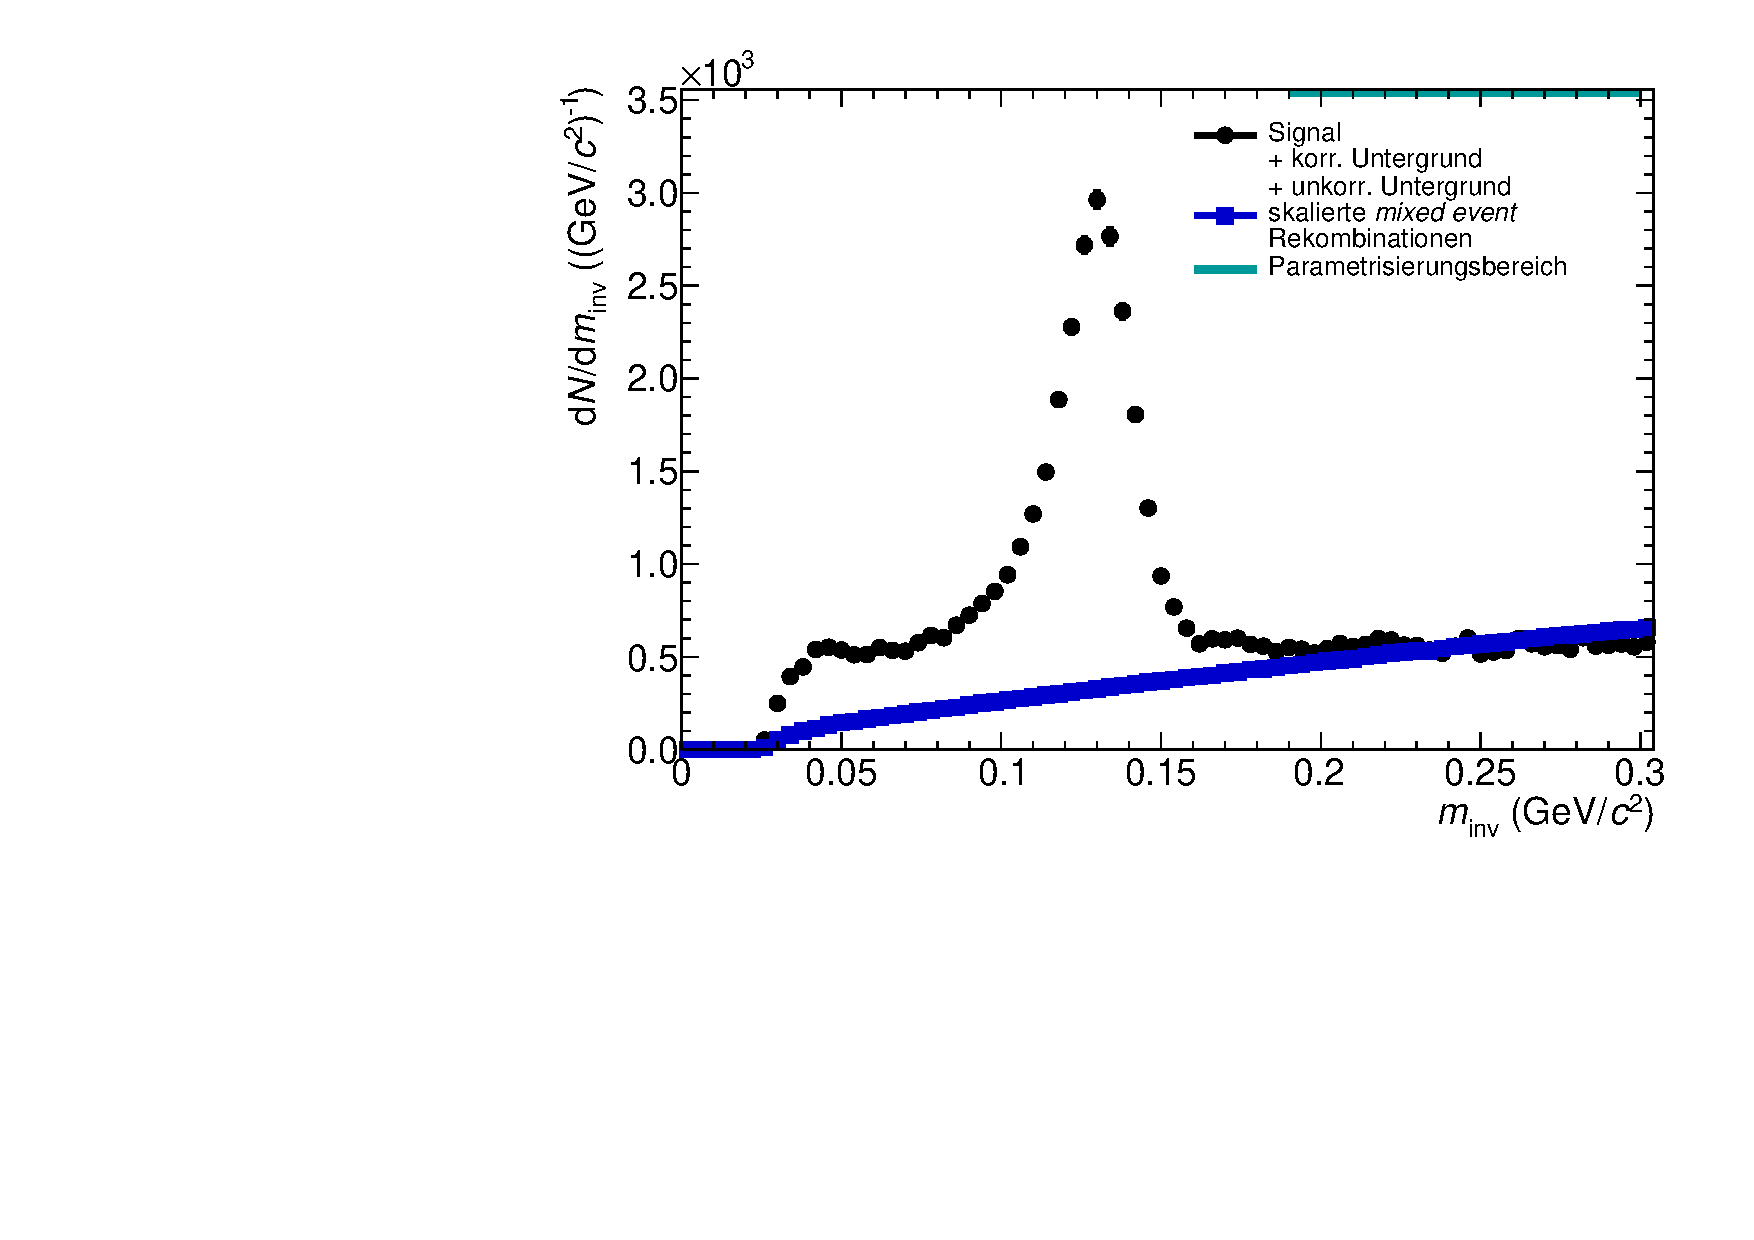
\includegraphics[width=.7\linewidth]{hUncorrBkgNorm.pdf}
		\caption{Nach Gleichung \ref{eqBackSkalierung} skalierte {\it mixed event} Rekombinationen aus Abbildung \ref{figUncorrBkg} als Absch{\"a}tzung des unkorrelierten Untergrunds zusammen aufgetragen mit Signal zuz{\"u}glich beiden Untergrundkomponenten (Abbildung \ref{figSignalPlusBkg}).}
		\label{figUncorrBkgNorm}
	\end{figure}
	Das Resultat der Skalierung ist in Abbildung \ref{figUncorrBkgNorm} zu sehen, wo zus{\"a}tzlich noch das Signal inklusiver beider Untergr{\"u}nde eingezeichnet ist, um besser erkennen zu k{\"o}nnen, wie sich der abgesch{\"a}tzte korrelierte Untergrund relativ zum gesamten Signal verh{\"a}lt.
	Das es sich hierbei nur um eine Absch{\"a}tzung handelt kann daran ausmachen werden, dass um $m_{inv} = 0.3 (\text{GeV/}c)$ der unkorrelierte Untergrund gr{\"o}{\ss}er ist, als das Signal mit beiden Untergrundkomponenten, was bedeutet, dass nach Abzug des unkorrelierten Untergrunds das Signal mit korreliertem Untergrund dort negativ w{\"a}re, was physikalisch nicht sinnvoll ist.
	\subsubsection{Absch{\"a}tzung des korrelierten Untergrunds}
	\subsection{Peak Extraktion mit Templates}
	\subsubsection{Templates}
	\subsubsection{Fit Methode}
	\section{Korrigierter Yield}
	\subsection{Korrekturen}
	\subsection{Variationen}
	\section{Zusammenfassung und Aussicht}



\end{document}
